\section{Описание}

Результатом лабораторной работы является отчёт, состоящий из:\\


    \quad1. Дневника выполнения работы, в котором отражено что и когда делалось, какие средства использовались и какие результаты были достигнуты на каждом шаге выполнения лабораторной работы.
\newline

    \quad2. Выводов о найденных недочётах.
\newline

    \quad3. Общих выводов о выполнении лабораторной работы, полученном опыте.


\section{Дневник выполнения работы}


Основные этапы создания программы:\\


    \quad1. Реализация необходимых алгоритмов.
\newline

    \quad2. Выявление логических ошибок в коде программы.
\newline

    \quad3. Выявление утечек памяти.
\newline

    \quad4. Выявление неэффективно работающих участков кода.

\section{Используемые средства}

\subsection{Valgrind}

Valgrind – это инструмент для отслеживания утечек памяти (и не только), который удобно использовать при работе с терминалом. Для его использования необходимо скомпилировать программу и вызвать valgrind от исполняемого файла. Эта утилита не только cообщит о наличии утечек, но и покажет, при исполнении какой функции они произошли. Valgrind сам подсказывает, какие ключи использовать для более наглядного отчёта об ошибках.


\begin{verbatim}
root@DESKTOP-5HM2HTK:~# valgrind ./a.out <tests/1.t
==1305== Memcheck, a memory error detector
==1305== Copyright (C) 2002-2017, and GNU GPL'd, by Julian Seward et al.
==1305== Using Valgrind-3.15.0 and LibVEX; rerun with -h for copyright info
==1305== Command: ./a.out
==1305==
...
==1301==
==1301== HEAP SUMMARY:
==1301==     in use at exit: 122,880 bytes in 6 blocks
==1301==   total heap usage: 39,358 allocs, 39,352 frees, 3,028,856 bytes allocated
==1301==
==1301== LEAK SUMMARY:
==1301==    definitely lost: 0 bytes in 0 blocks
==1301==    indirectly lost: 0 bytes in 0 blocks
==1301==      possibly lost: 0 bytes in 0 blocks
==1301==    still reachable: 122,880 bytes in 6 blocks
==1301==         suppressed: 0 bytes in 0 blocks
==1301== Rerun with --leak-check=full to see details of leaked memory
==1301==
==1301== For lists of detected and suppressed errors, rerun with: -s
==1301== ERROR SUMMARY: 0 errors from 0 contexts (suppressed: 0 from 0)
root@DESKTOP-5HM2HTK:~#
\end{verbatim}

Как видно из сводки valgrind, моя программа очищает всю задействованную оперативную память даже на больших входных данных.

\subsection{Callgrind}
Эта утилита входит в состав инструмента valgrind. Она эмулирует
каждую исполняемую инструкцию программы и на основании внутренних метрик о «стоимости» работы каждой инструкции выдает нужное нам заключение.

Чтобы использовать утилиту сallgrind, нужно собрать программу с ключами -g и -no-pie. В папке запуска сгенерируется отчёт c именем «callgrind.out.<номер$\textunderscore$процесса>». Чтобы можно было быстро работать с отчётом, была задействована программа KCachegrind. При выборе нужной функции, на экране отобразится цепочка функций, вызывающих выбраную и вызываемых выбранной. \\
Граф для моей реализации дерева:

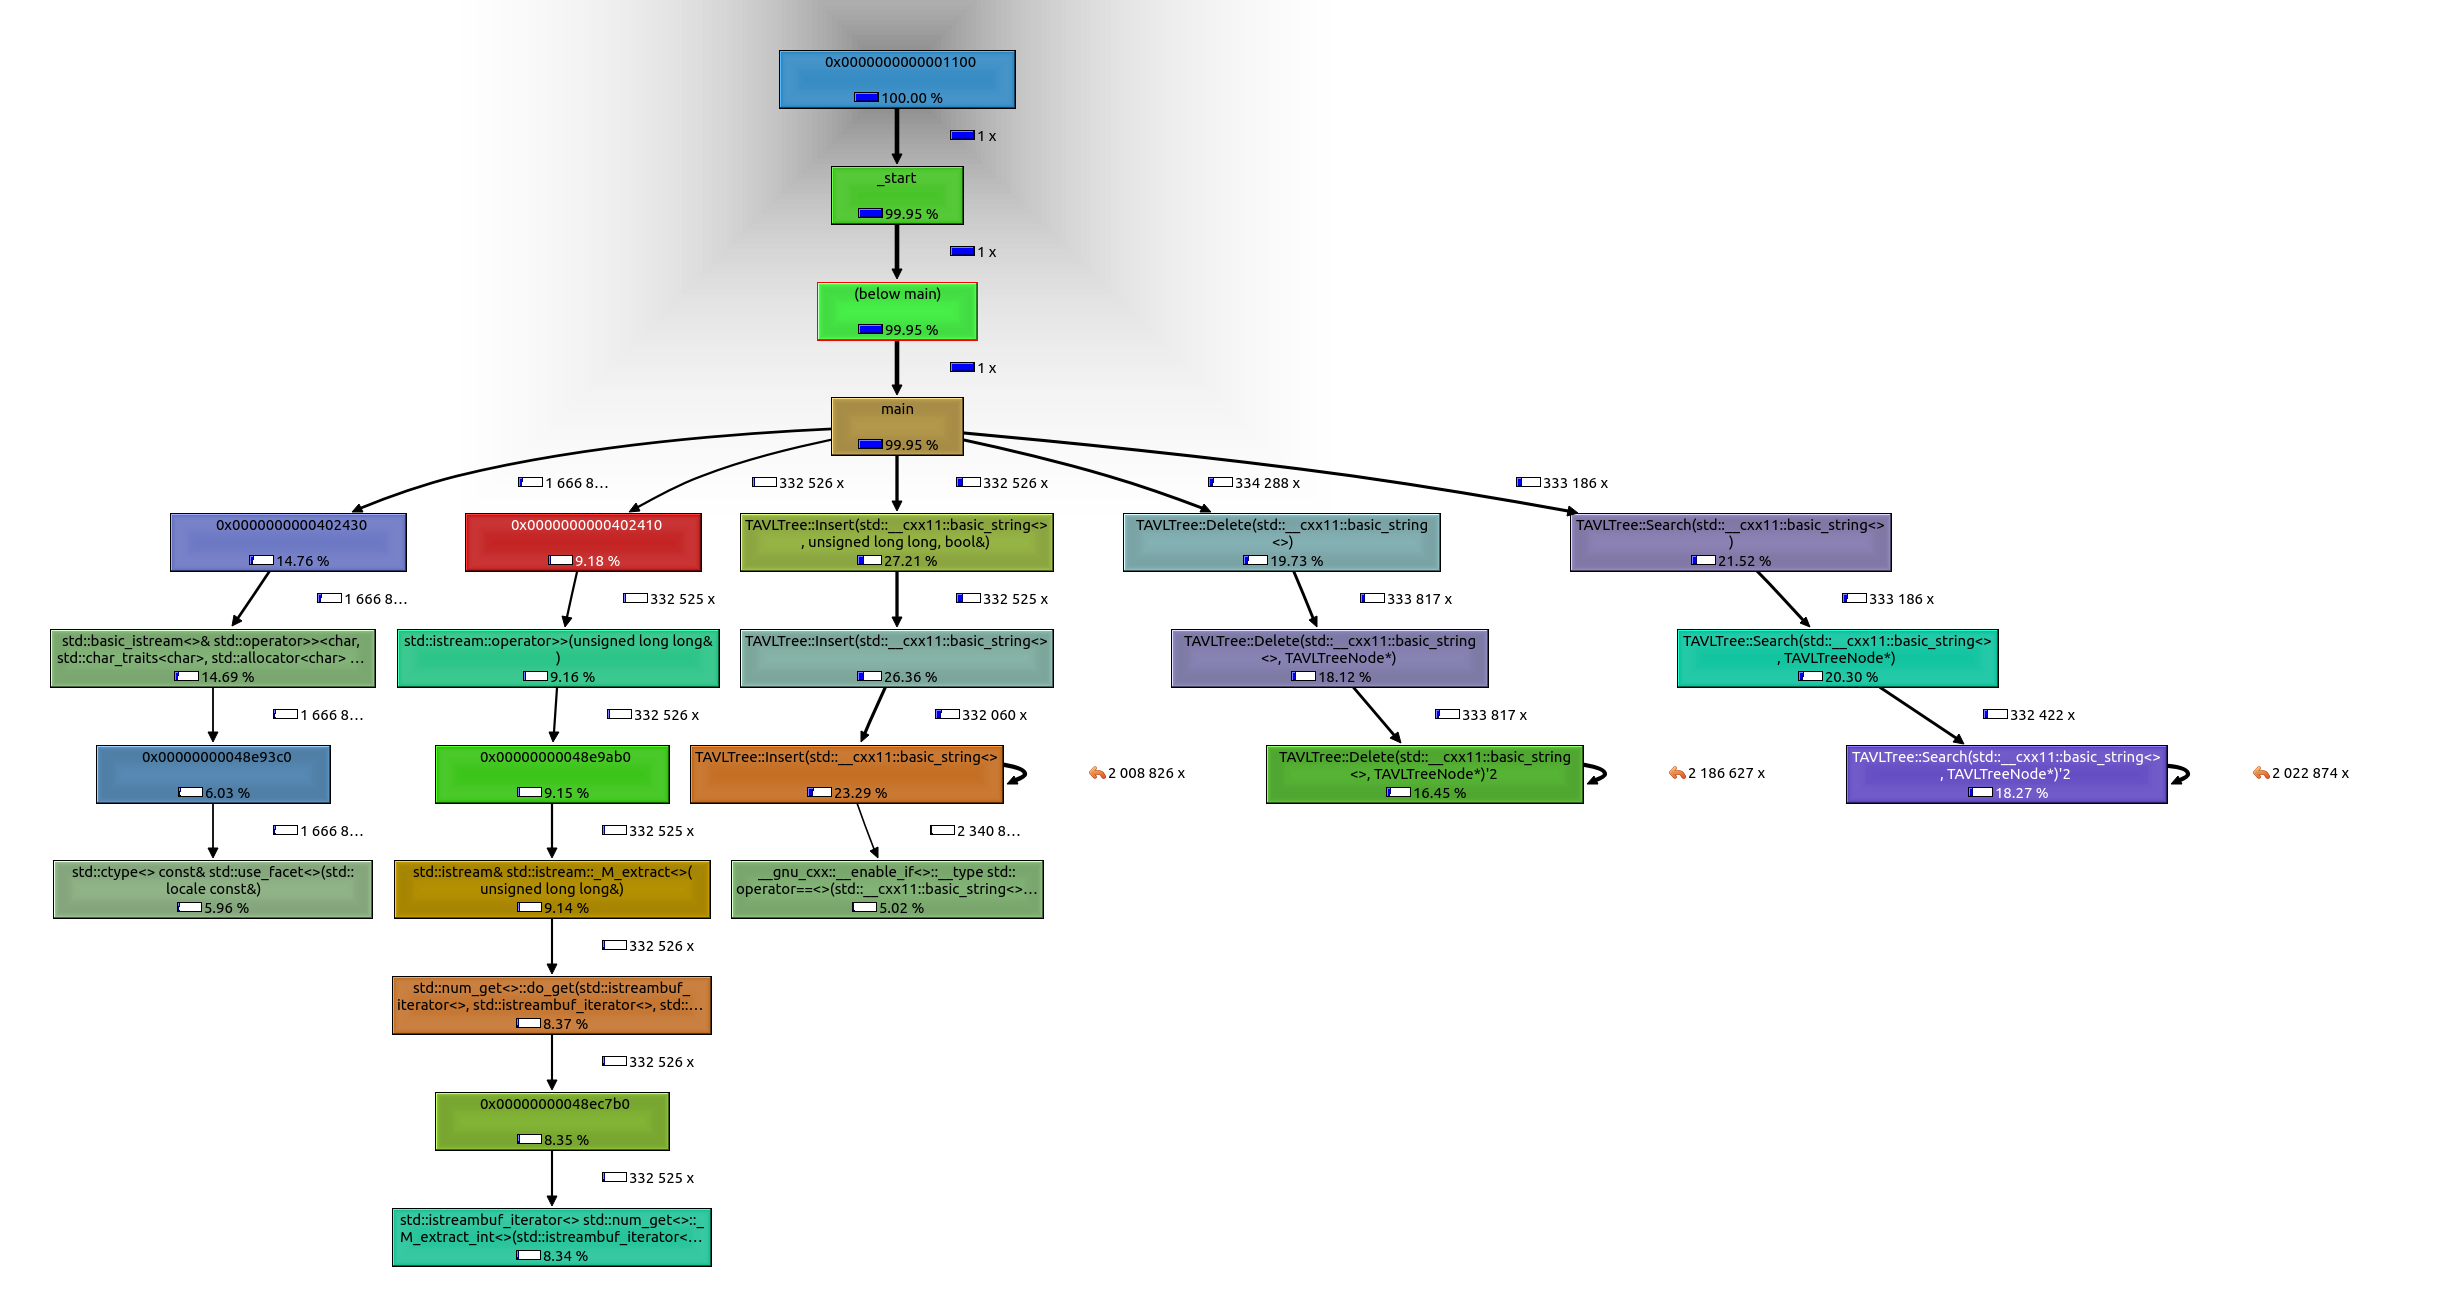
\includegraphics[width=7.5in,height=150mm]{src/graph.png}

По нему мы можем заметить, что больше всего времени тратиться для выполнения функции добавления в дерево. Это связано с тем, что при добавлении элемента в $AVL-$дерево происходит ребалансировка, которая требует дополнительного времени.


\subsection{Gprof}
Профилировщик от google работает по другому принципу. Вместо того, чтобы анализировать каждую инструкцию исполняемой программы, он приостанавливает выполнение программы через равные промежутки времени и пытается определить, в какой функции в данный момент находится за счёт раскрутки стека. В результате, это почти не влияет на производительность запущенного приложения. Но у такого подхода есть и свои слабые стороны. Для удобства анализа полученного отчёта можно его преобразовать в графическую форму с помощью утилиты gprof2dot, которая может преобразовывать его в формат .png или .svg.

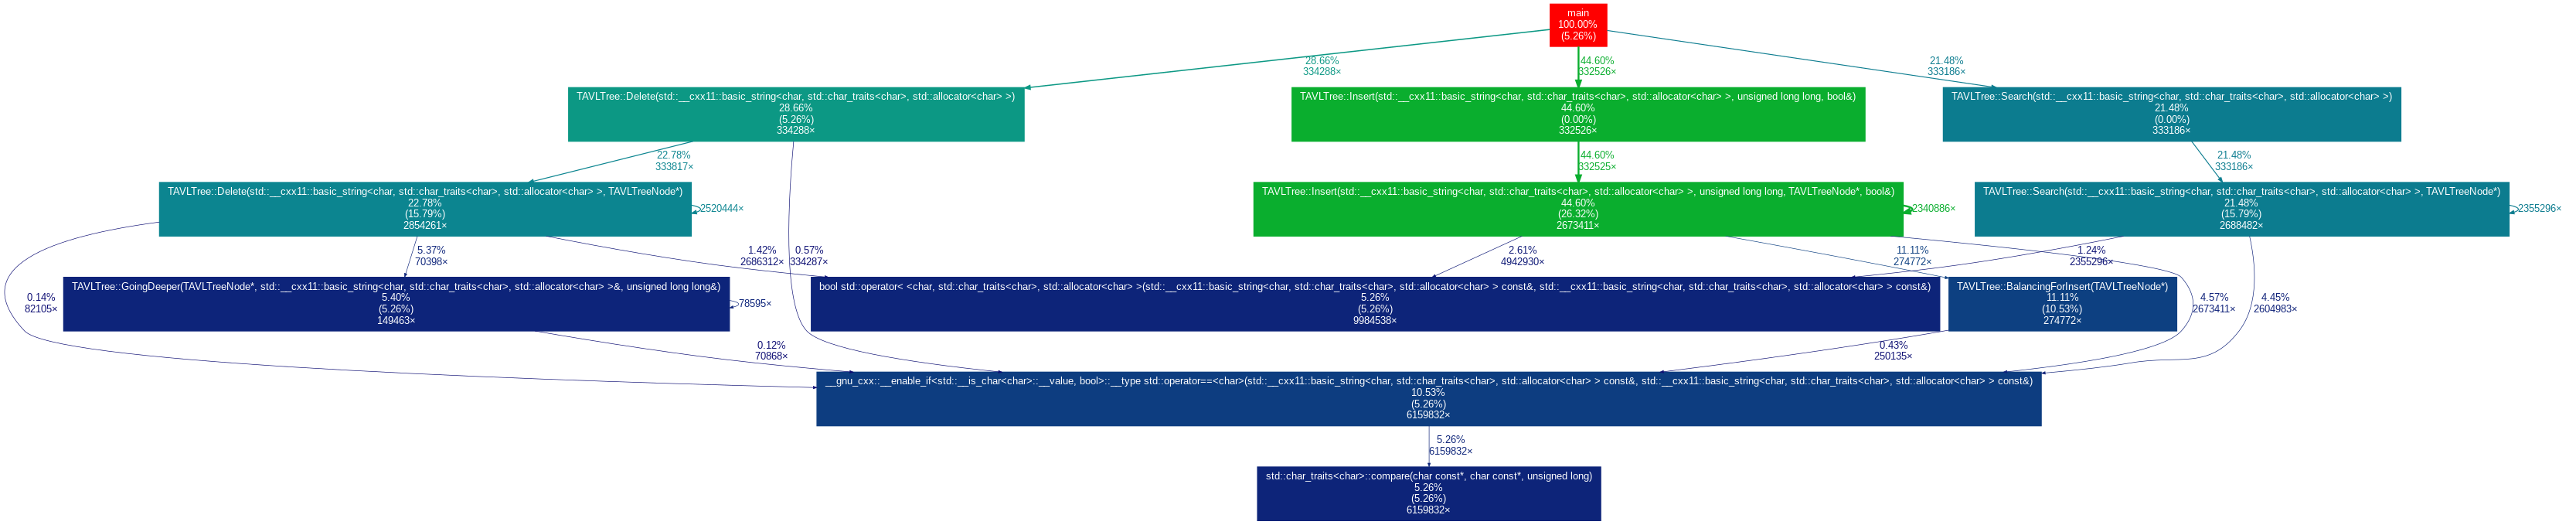
\includegraphics[width=7in,height=70mm]{src/output.png}

Полученное дерево в результате работы этой программы показывает примерно те же результаты. Функция добавления по-прежнему занимает больше времени, чем другие функции. В данном отчёте gprof включил работу аллокатора и некоторых других функций в работы основных трёх функций: удаление элемента, добавление элемента и поиск.



\pagebreak

